\documentclass{article}

\usepackage[portuguese]{babel}

\usepackage{amsmath, amssymb}
\usepackage{graphicx}
\usepackage[colorlinks=true, allcolors=blue]{hyperref}

\usepackage[section]{placeins}

\title{Atividade em aula 04}
\author{Vinícius de Oliveira Peixoto Rodrigues (245294)}
\date{Agosto de 2022}

\begin{document}
\maketitle

\section*{Exercício 01}
\subsection*{Item (a)}

A especificação constrói um lexer que conta o número de palavras (\texttt{p}), linhas (\texttt{l}) e caracteres (\texttt{c}) do input.

\subsection*{Item (b)}
\begin{figure}[!ht]
    \begin{center}
        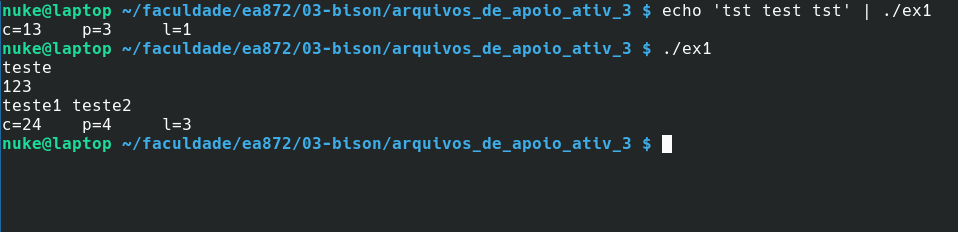
\includegraphics[width=\textwidth]{images/ex1_b.png}
        \caption{Exemplo de funcionamento do lexer \texttt{ex1}}
    \end{center}
\end{figure} 

\subsection*{Item (c)}

Ela guarda o comprimento da string na qual o \texttt{flex} deu match de acordo com alguma das regras definidas. Está sendo usada para contar o número de caracteres (incluindo espaços em branco, tabs, newlines e EOF).

\subsection*{Item (d)}

Serve para dar match em caracteres que não são um whitespace, um \texttt{"\textbackslash n"} (newline) ou um \texttt{"\textbackslash t"} (tab).

\subsection*{Item (e)}

Porque ela permite levar em conta os caracteres do grupo do item (c) na contagem de caracteres total do input.

\section*{Exercício 2}

\subsection*{Item (a)}

Ela inclui o header gerado automaticamente pelo bison (\texttt{ex2.tab.h}) que contém declarações de variáveis e funções do bison que o lexer faz uso (em particular o \texttt{yylval}).

\subsection*{Item (b)}

\begin{itemize}
    \item \texttt{yytext}: é onde o lexer guarda os tokens (como strings) que são extraídos da entrada
    \item \texttt{yylval}: é a variável através da qual o lexer informa o valor \textbf{semântico} de um token para o parser (nesse caso o valor numérico do número hexadecimal lido)
\end{itemize}

\section*{Item (c)}

\begin{itemize}
    \item \texttt{\$\$}: serve para guardar o resultado da resolução de uma regra
    \item \texttt{\$1}: serve para se referir ao valor do elemento de posição 1 em uma regra
    \item \texttt{\$2}: serve para se referir ao valor do elemento de posição 2 em uma regra
\end{itemize}

\section*{Item (d)}

O lexer passa o valor do número hexadecimal lido para a global \texttt{yylval}, que em seguida é usado para resolver o \texttt{linha} na regra \texttt{linhas: linhas linha}, e só então ele é impresso.

\section*{Item (e)}

É necessário porque a regra de resolução \texttt{linha : INTEIRO '\textbackslash n'} exige o newline após o token. Se a linha não estivesse presente, o parser não resolveria a regra \texttt{linha} e os números não seriam parseados, gerando erro de sintaxe.

\section*{Exercício 3}

\subsection*{Item (a)}

Uma sequência de dígitos com tamanho maior ou igual a 0, seguida por um ponto, seguida por uma sequência de dígitos de tamanho maior ou igual a 0.

\subsection*{Item (b)}

A sequência que contém só um ponto final, \texttt{"."}, é aceita como um número float válido. Para corrigir isso, basta colocar a restrição de que é necessário ter dígitos de pelo menos um dos dois lados:

\begin{verbatim}
    frac    [0-9]*([0-9]\.?|\.[0-9])[0-9]*
\end{verbatim}

\subsection*{Item (c)}

Basta criar uma nova definição:

\begin{verbatim}
    hex     0x[0-9a-zA-Z]+
\end{verbatim}

e então criar uma regra do lexer:

\begin{verbatim}
    {hex}   {
                sscanf(yytext, "%x", &yylval.valor_inteiro);
                return INTEIRO;
            }
\end{verbatim}

\begin{figure}[!ht]
    \begin{center}
        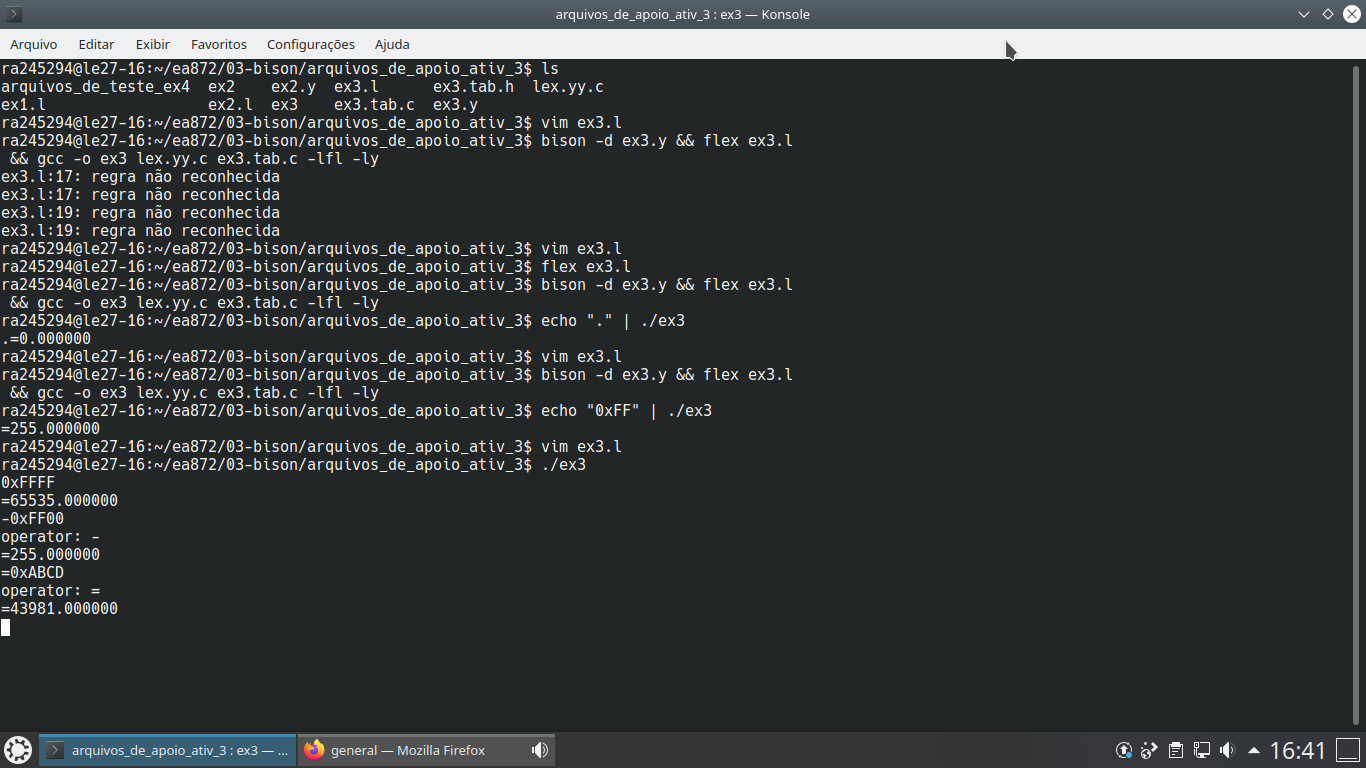
\includegraphics[width=\textwidth]{images/ex3_c_2.png}
        \caption{Exemplo de funcionamento do lexer \texttt{ex3}}
    \end{center}
\end{figure} 

\begin{figure}[!ht]
    \begin{center}
        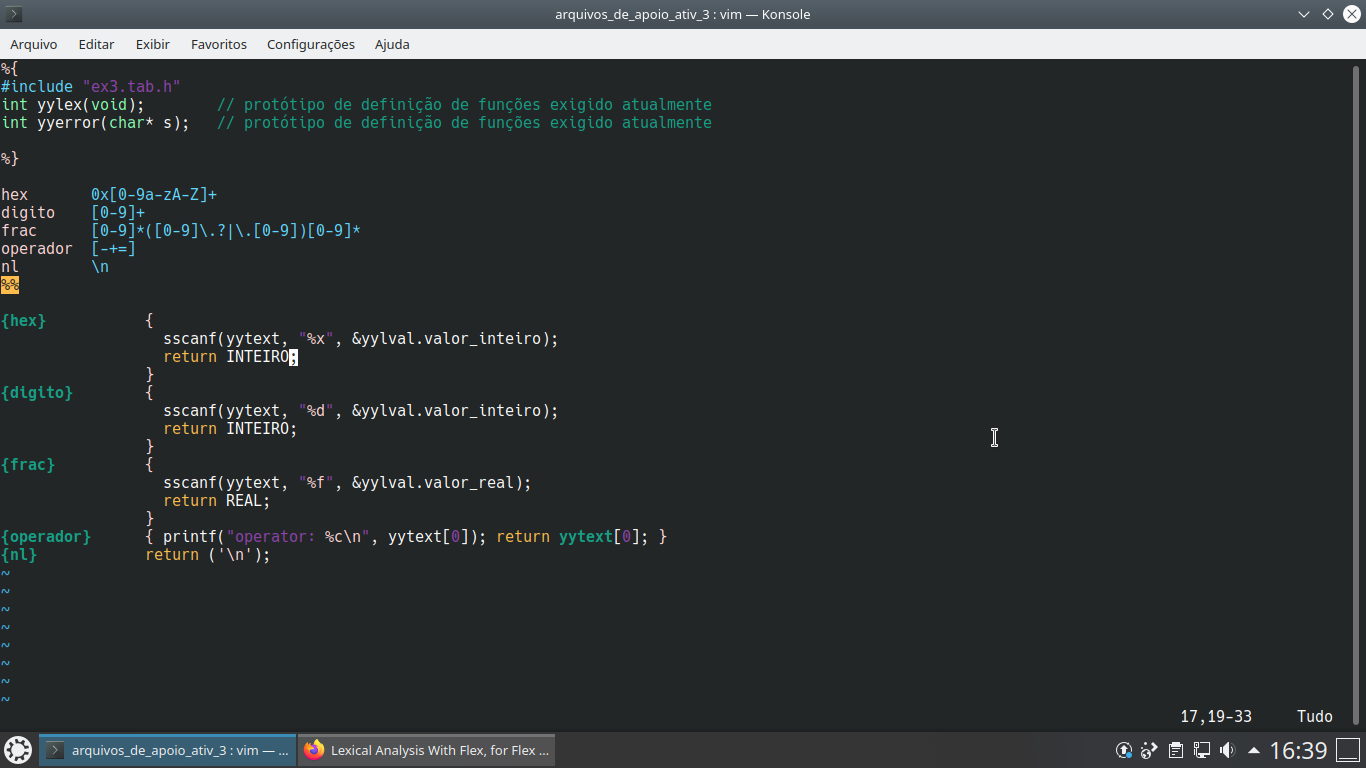
\includegraphics[width=\textwidth]{images/ex3_c_1.png}
        \caption{Exemplo de funcionamento do lexer \texttt{ex3}}
    \end{center}
\end{figure} 
\end{document}